\chapter{构建垫片三维模型}\label{chap:dianpian}

{\bfseries 学习目标}
\begin{itemize}
\item 学习利用layer命令管理图层和设置图线
\item 学习利用xline命令绘制辅助线
\item 学习利用arrayploay建立环形阵列
\item 学习利用cylinder命令进行圆柱体的三维建模
\item 学习利用3darray建立三维物体环形阵列
\item 掌握平面图形分析的基本方法
\end{itemize}

{\bfseries 任务要求}
\begin{itemize}
\item 根据图\ref{fig:tiaoyafadianpian}所示的零件图,用旋转法建立调压阀垫片零件的三维模型
\item 根据图\ref{fig:tiaoyafadianpian}所示的零件图,用拉伸法建立调压阀垫片零件的三维模型
\item 根据图\ref{fig:tiaoyafadianpian}所示的零件图,用实体建模法建立调压阀垫片零件的三维模型
\end{itemize}

\noindent
\begin{figure}[htbp]
\centering
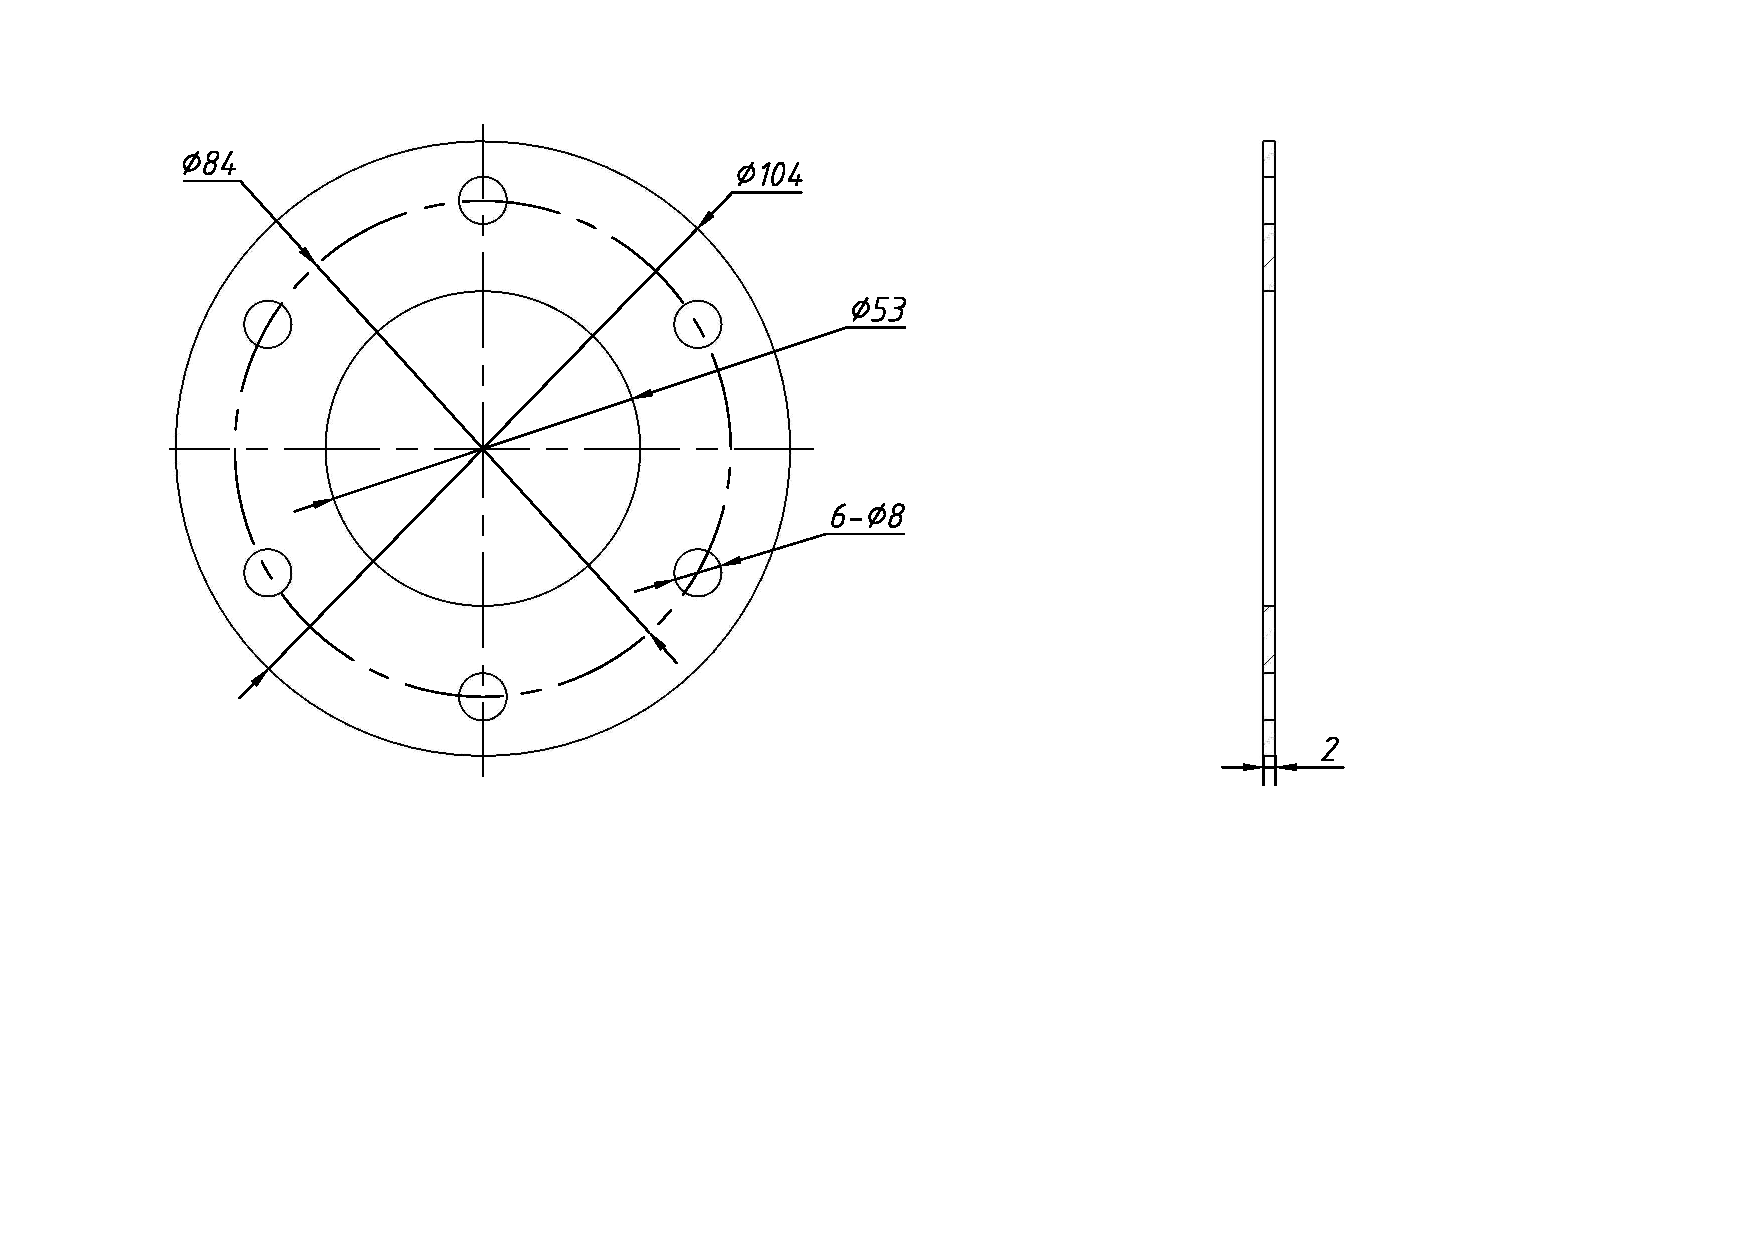
\includegraphics[scale=0.6]{tiaoyafadianpian.pdf}
\caption{垫片零件图}\label{fig:tiaoyafadianpian}
\end{figure}

\endinput